\clearpage
\section{Step 3: Code Quality Analysis}
    In this section, the quality of the code will be analysed.
    To aid us in the process, we will use the tool called SonarQube.
    \footnote{SonarQube official website: \url{https://www.sonarqube.org/} }.\\\\
    \textbf{Note:}
    \begin{adjustwidth}{1cm}{}
        The Optaplanner source code is spread into multiple packages that serve different purposes. For example, the package called \cb{optaplanner-core} contains the source code of the implementation of the algorithms that OptaPlanner uses, together with all the data necessary for the algorithms to run. We consider this the most important package for the project, and our analysis will be mainly focused on it. Other packages, such as \cb{optaplanner-examples}, contain examples of how the code in the \cb{core} package can be used, while the \cb{optaplanner-benchmark} can be used to analyse the scores obtained by the algorithms. \\
        Throughout our analysis, we will look at the overall metrics of the project, but the \cb{optaplanner-core} package will be analysed more thoroughly.
    \end{adjustwidth}
    
    \subsection{SonarQube}
        According to the official documentation:\\
        \begin{adjustwidth}{1.5cm}{}
            \textit{SonarQube is an automatic code review tool that detects bugs, vulnerabilities and code smells 
            in code. It can integrate with the existing workflow to enable continuous code inspection
            across the project branches and pull requests.}
        \end{adjustwidth}
        \vspace{0.5cm}
        From this description we can conclude that this tool is fit for our analysis and that it will aid us with inspecting the source code of the OptaPlanner project. At the same time, a big advantage that it brings is that the tool can integrate with existing workflows - meaning that it is integrated with Maven, making the tool even easier to use for our case. \\
        The following sections will document the findings of the tool when used to inspect OptaPlanner.
        
    \subsection{Method of analysis}
        Using SonarQube, we will analyse the quality of the code for our project.\\
        OptaPlanner can be built using Maven 
        \footnote{Maven official website: \url{https://maven.apache.org/}},
        a build automation tool used primarily for Java projects. As such, we can make use of the fact that SonarQube is compatible with Maven, and we will run the tool through Maven. The project first needs to be compiled through Maven, using the following command which is also described in the documentation:
        \begin{lstlisting}
$ mvn clean install -Dskiptests\end{lstlisting}
        Running SonarQube is straightforward. In order to have it analyse our software, we need to run it inside the project folder containing the \texttt{pom.xml} file with the following command:
        \begin{lstlisting}
$ mvn sonar:sonar 
    -Dsonar.projectKey=OptaPlanner 
    -Dsonar.host.url=http://localhost:9000 
    -Dsonar.login=token\end{lstlisting}
        By running this command, SonarQube analyses the structure of the code by looking at the objects compiled by Maven. 
        In the argument list, authentication credentials need to be provided, and in our case, we have used the token generated by SonarQube.\\\\
        The results of the analysis can then be seen in the web interface of SonarQube, when they are finished loading after running the before mentioned command. Figure \ref{fig:sonarqube_ss} shows how the results are displayed for our software, when analysing the entire code base, including all the packages.
        \begin{figure}[H]
            \centering
            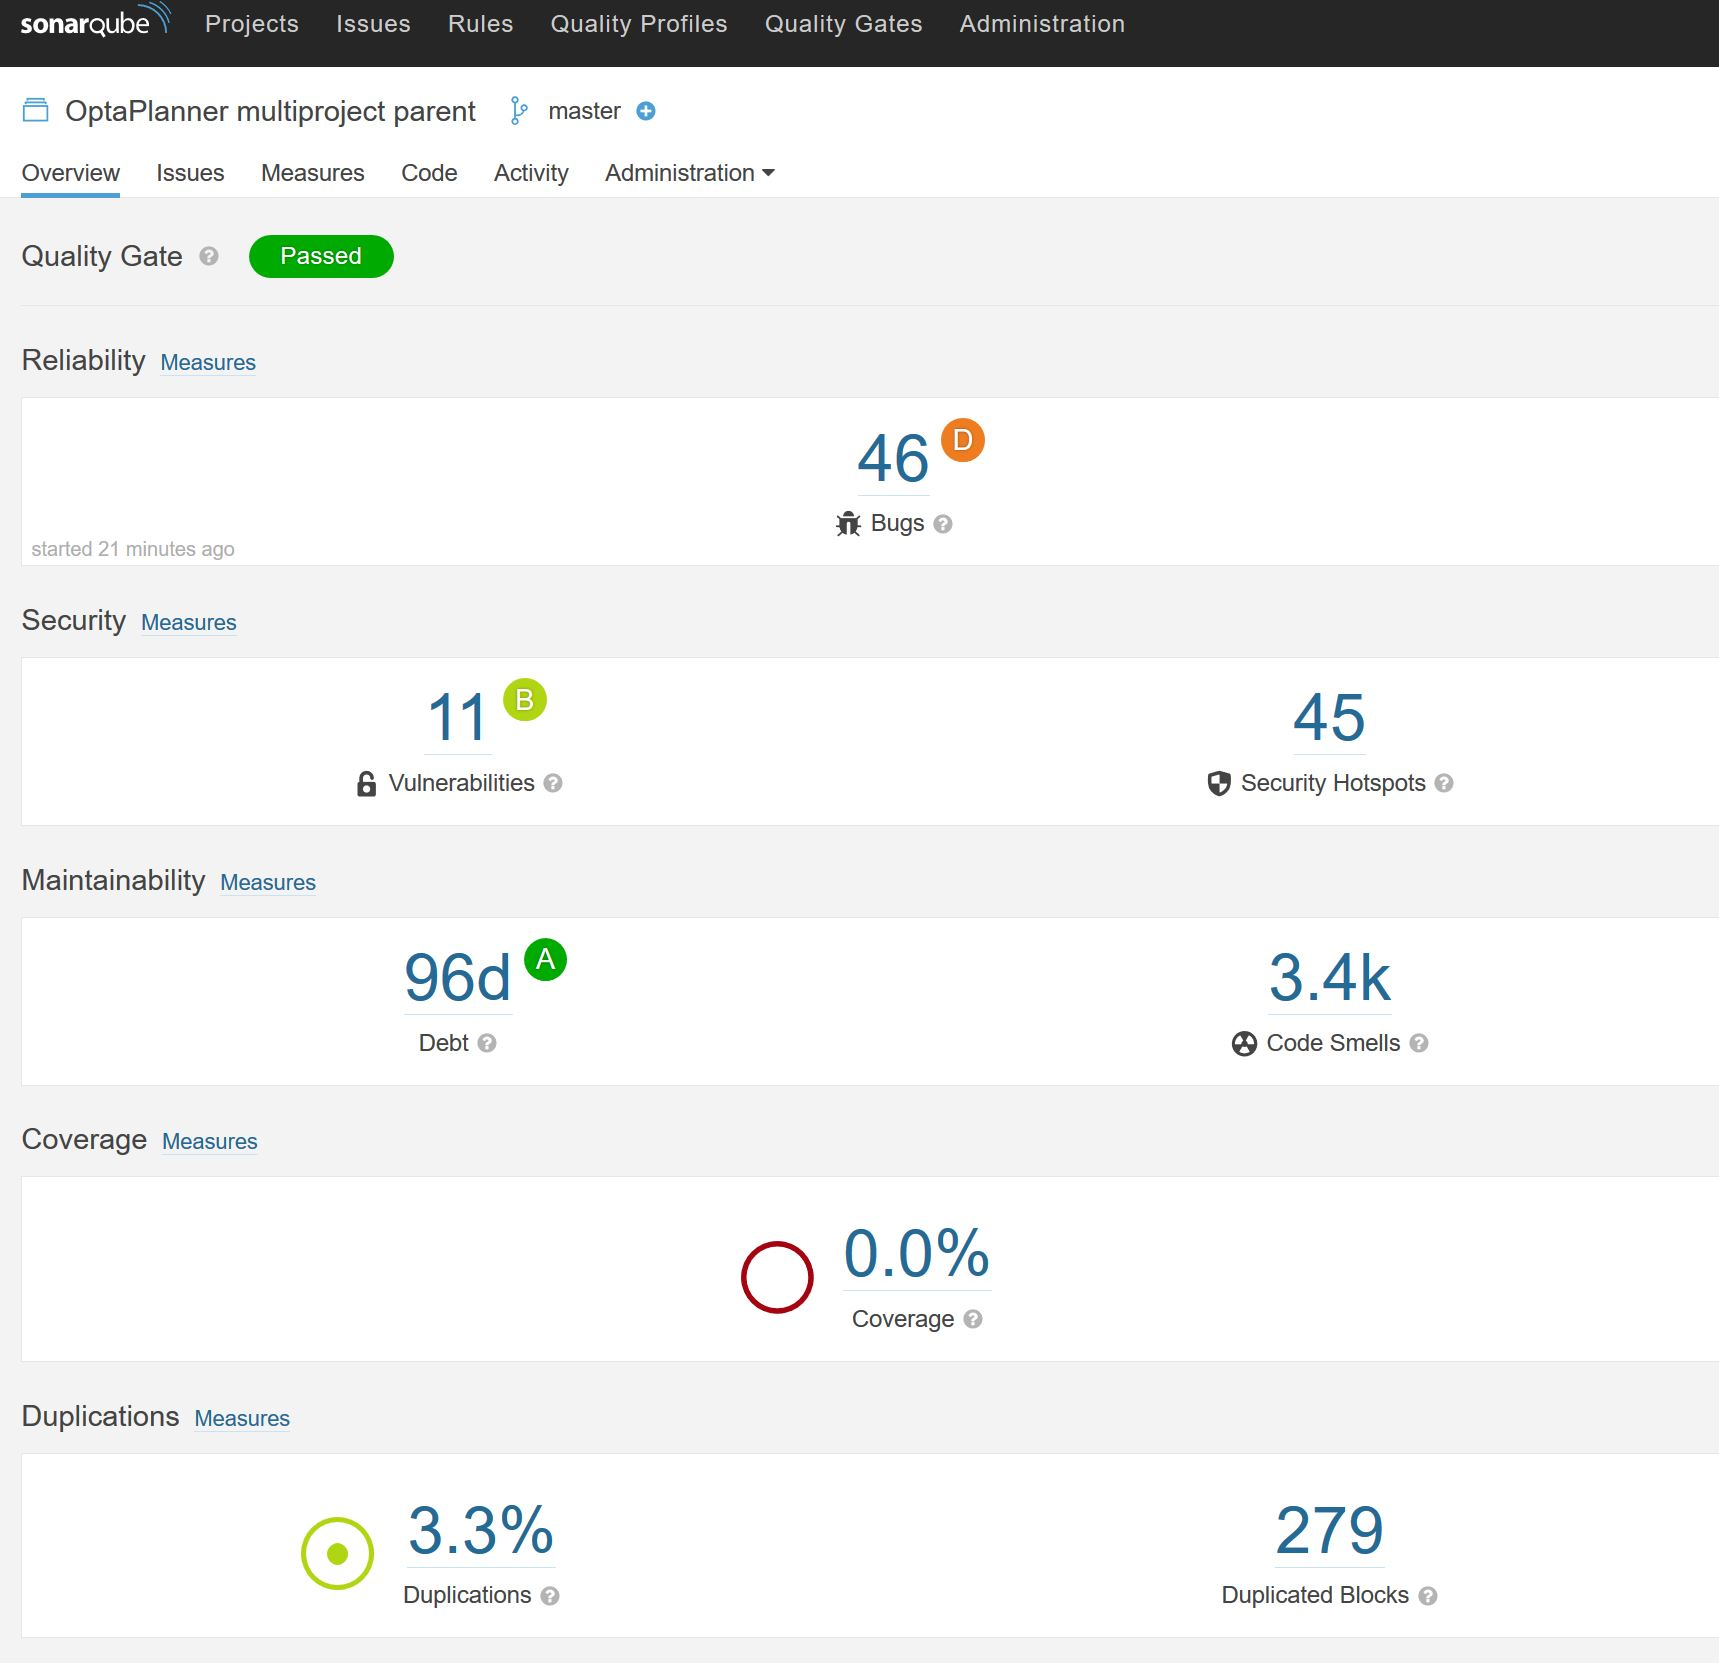
\includegraphics[scale=0.7]{figures/sonarqube_ss.JPG}
            \caption{Web interface of the SonarQube report of OptaPlanner}
            \label{fig:sonarqube_ss}
        \end{figure}
        At the first glance, the tool tells us that the project's Quality Gate is Passed, which means that the project is production-ready. If this was not the case, the developers should first look into the issues that cause this, fix them, and then re-run the analysis to see if there has been an improvement. This Quality Gate is, according to the documentation, a Boolean value, meaning that a project is either stable enough to be deployed or it is not.\\\\
        The tool presents us with a list of  measures, for attributes such as Reliability and Maintainability. It also shows the percentage of the code that has been found as a duplicate (identical lines of code) - in our case, 3.3\% of the total code is a duplicate. 
        Each measure will be briefly analysed in the following sections. 
    
    \subsection{Metrics}
        In this section, we will give in-depth explanations of the metrics that have been found using SonarQube, together with our interpretations as to why these results have been found. The following sections will document specific metrics individually.
        
        \subsubsection{Size metrics}
            OptaPlanner is a project of substantial size, in terms of packages, classes and lines of code. According to the analysis tool, the following metrics have been found:
            \begin{itemize}
                \item \textbf{Lines of code and files} \\
                In total, the project has 105,792 lines of code contained in 1,535 files, which are unevenly spread between the packages. Out of them, 104,000 are written in Java, and the rest in XML. By looking deeper into the project, the tool provides us with the following insights:
                    \begin{itemize}
                        \item[-] The biggest package is \cb{optaplanner-core}, containing 52,818 LOCs in 845 files. \\ 
                        Out of the three main components of this package, the \cb{impl} folder is the biggest one, with 37,086 LOCs and 633. The other two main components, \cb{config} and \cb{api} have 8.5k and 7k LOC respectively, however, the \cb{api} folder has 141 files, twice as many as \cb{config}, with 70.
                        The difference in size between those three packages was to be expected, since the biggest folder contains all the implementation details of the algorithms, while the other two are only concerned with the interfaces to the implementation.\\
                        In this package, the file with the most LOCs has 1048, and can be found at: \\ 
                        \cb{core/impl/domain/solution/descriptor/SolutionDescriptor.java}. \\
                        This number is very high, making this a very long class compared to the rest of the project, where most files have under 200 LOCs.\\\\
                        An overview of the LOC in the \cb{core} folder can be seen in Figure \ref{fig:loccore}
                        \begin{figure}[H]
                            \centering
                            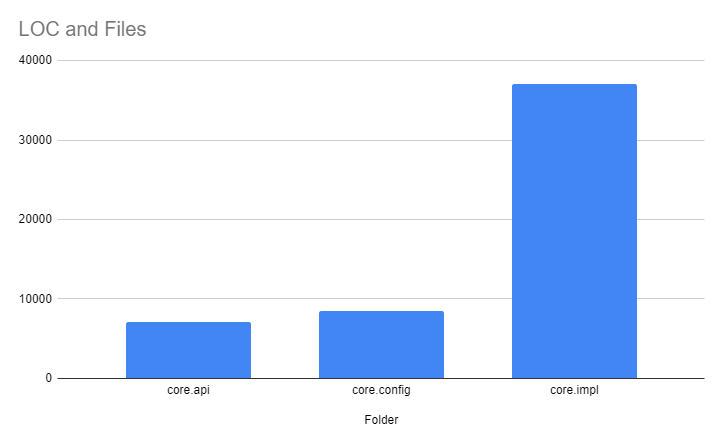
\includegraphics[scale=0.6]{figures/step3/locfiles.PNG}
                            \caption{LOC in \cb{core}}
                            \label{fig:loccore}
                        \end{figure}
                        \item[-] The second biggest package is 
                        \cb{optaplanner-examples} with 41,450 LOCs; out of the 22 examples, the Conference Scheduling
                        \footnote{\url{https://docs.optaplanner.org/7.32.0.Final/optaplanner-docs/html\_single/index.html\#conferenceScheduling}}
                        and Nurse Rostering
                        \footnote{\url{https://docs.optaplanner.org/7.32.0.Final/optaplanner-docs/html\_single/index.html\#nurseRostering}}
                        stood out as the biggest, with 4,262 and 3,460 LOC respectively.
                    \end{itemize}
                \item \textbf{Statements}\\
                    The project contains in total 41,169 statements. As expected from the previous metric, the package with most statements is the \cb{optaplanner-core} one, with 18,692, followed by the \cb{optaplanner-examples} package with 18,291. \\ 
                    The file with the most statements is the one that also has the most LOC, namely \\
                    \cb{core/impl/domain/solution/descriptor/SolutionDescriptor.java}. This file contains 496 statements, a considerably high number taking into consideration that most files have around ~100 statements, with a very small number of them going over 100.
                    \\ \textcolor{red}{TODO: maybe add some graphs here? might be nice to see}
                    
                \item \textbf{Functions}\\
                    The \cb{optaplanner-core} package has a total of 6500 functions. Out of its three main components, the \cb{impl} one is the biggest, with 4479 functions, followed by \cb{api} with 1112 and \cb{config} with 909. The biggest file is still the \cb{SolutionDescriptor.java}, with 64 functions.
                \item \textbf{Classes}\\
                    The most classes are contained in the same package, with a total of 861, with the \cb{impl} folder containing 674, \cb{api} with 116 and \cb{config} with 71. \\
                    Most of the files in the project contain one class, indicating a good design since having too many classes declared in a single file could be a potential code smell (more about this later on). However, one folder stood out where most files contained 2 or 3 classes. In the following folder
                    \\ \cb{core/impl/domain/valuerange/buildin/composite/}, most files contain more than one class. This is due to the fact that the developers needed a way to enrich the basic types in Java with extra information, and created their own Object types from the standard ones. 
                    \\ For example, the file \cb{core/impl/domain/valuerange/buildin/primint/IntValueRange.java} contains three classes used to iterate through the elements in a specific interval of integer values. 
                \item \textbf{Comment lines}\\
                    The \cb{optaplanner-core} package contains 8,007 comment lines, taking up 13.2\% of the total size of the code. Unlike the other metrics mentioned above, the component with the most comments is the \cb{api} one, with 4,303, followed by \cb{impl}. This is due to the fact that the APIs are the interfaces that connect the implementation of the software with the 'outside world'. They are the point of communication for the other developers, and as such, need to be properly explained and documented so that they can be understood by the developers who do not know about the inner workings of the system. Having well documented and commented APIs is a great advantage and helps a lot with our key drivers of Maintainability and Integrability, since they allow the system to be easily used, maintained and integrated without having to first study the code or the implementation that lies within.
            \end{itemize}
            From the size analysis, it is quite clear that the biggest folder is \cb{optaplanner-core/impl}, which contains the most LOC, most functions and statements and the most files. This was to be expected, since this folder contains the implementation details of the software, thus the implementation of the algorithms that are the foundation of the project. The fact that the developers have implemented these complex algorithms themselves explains the big size of the folder; moreover, they focused also on optimization and performance, so the algorithms can be tweaked and adapted to a high number of situations. As such, a lot of work in terms of LOC needed to be done to achieve this.
        
        \subsubsection{Complexity}
            SonarQube can, according to the documentation, analyse two types of complexity metrics: 
            \begin{itemize}
                \item \textbf{Cyclomatic complexity} \\
                \textit{Measures the minimum number of test cases required for full test coverage}.\\ Optaplanner has a cyclomatic complexity of 19733. As expected, the \cb{optaplanner-core} package is the most complex, with a score of 10,307.\\
                By further exploring the package, we have come across the following scores:
                \begin{itemize}
                    \item[-] The \cb{impl} folder is the most complex, with a score of almost 7000. Again, this is expected, since this component is the biggest and the most important for the project. 
                    \item[-] The complexity of the other two packages is 1483 for \cb{api} and 1855 for \cb{config}.\\
                    An overview of the three folders together with their complexities can be seen in Figure \ref{fig:corecyclomatic}
                    \begin{figure}[H]
                        \centering
                        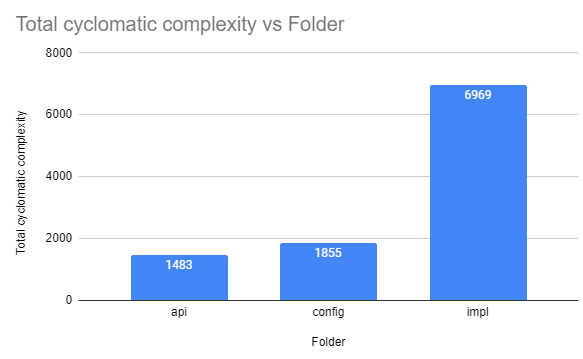
\includegraphics{figures/step3/cyclomaticcomplexitycore.PNG}
                        \caption{Total cyclomatic complexity of the folders in \cb{core}}
                        \label{fig:corecyclomatic}
                    \end{figure}
                    \item[-] In the \cb{impl} folder, the package with the highest complexity is \cb{score}, with a complexity of 2801. This component helps give a score (weight) to a computed solution, and the complexity of this task comes from the big number of constraints that need to be satisfied when solving a problem, and how well the solution fits the constraints. At the same time, the score needs to keep track at all times of the domain of the problem, the heuristics, the type of search that is being used, and so on. In order to do this, it makes use of other components to compute the score, making it highly complex.
                    \item[-] The next two most complex folders are \cb{heuristic} - 1566 and \cb{domain} - 1382. These two are components that the algorithms need in order to find an optimal solution, and they hold the information that is fed into the algorithms, as well as the details about how the algorithms should behave (what kind of search heuristic should be used, for example). Since these two components are crucial to the software, it was expected that they were also fairly complex. 
                    \item An overview of the components inside the \cb{core.impl} folder and their complexities can be seen in Figure
                    \begin{figure}[H]
                        \centering
                        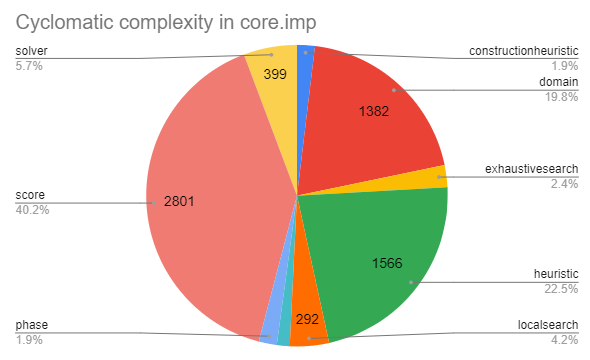
\includegraphics{figures/step3/cyclomaticcomplexityimpl.PNG}
                        \caption{Total cyclomatic complexity of the folders in \cb{core.impl}}
                        \label{fig:my_label}
                    \end{figure}
                \end{itemize}
                
                \item \textbf{Cognitive complexity}\\
                \textit{A measure of how difficult the project is to understand}.\\ The software has a cognitive complexity of 11849. The \cb{optaplanner-core} package is the most complex with a score of 5465.  
                By exploring the rest of the core package, we have come across the following scores:
                \begin{itemize}
                    \item[-] The \cb{impl} folder is the most complex, with a score of 3694. This is expected, since this component contains all of the functionality of the project; all the types of problems it can solve, the different solutions and so on. At the same time, it is also the biggest in terms of files and LOC. As such, we also expected this folder to be the most difficult to understand. 
                    
                    \item[-] The \cb{api} folder has a given complexity score of 608, the lowest of the three. This is also a good sign, since, mentioned before, this folder contains the interfaces that other parties can use in order to interact with the software. It should be as simple and as intuitive as possible, well documented and commented, to make the reuse of the other underlying code as easy and as fast as possible. The low complexity of these files could also positively influence maintainability. 
                    
                    \item[-] An overview of the complexity of the three folders can be seen in Figure \ref{fig:cognitivecomplexitycore}
                    \begin{figure}[H]
                        \centering
                        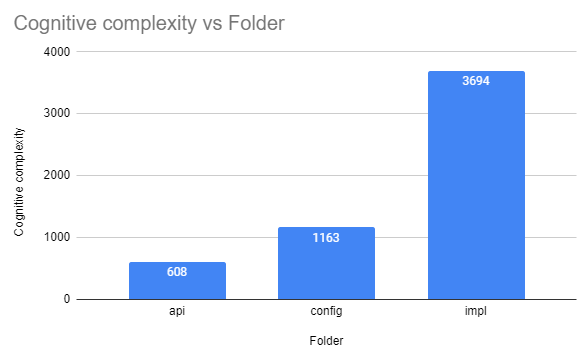
\includegraphics[scale=0.8]{figures/step3/cognitivcomplexitycore.PNG}
                        \caption{Cognitive complexity in \cb{core}}
                        \label{fig:cognitivecomplexitycore}
                    \end{figure}
                    
                    \item[-] Inside the \cb{impl} folder, the most complex components are \cb{domain}, \cb{heuristic} and \cb{score}. These are the same folders that also had a high cyclomatic complexity, and it was to be expected that they were also the most cognitively complex, with a score of around 1000 each. The same reasoning as before can be applied for this complexity as well.
                    
                    \item[-] An overview of the components inside the \cb{core.impl} folder can be seen in Figure \ref{cognitivecomplexityimpl}
                    \begin{figure}[H]
                        \centering
                        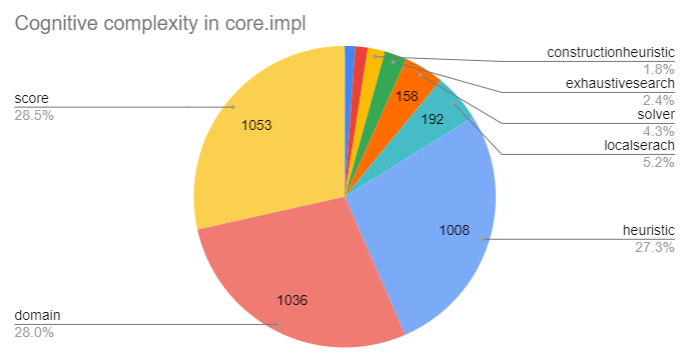
\includegraphics[scale=0.8]{figures/step3/cognitivecomplexityimpl.PNG}
                        \caption{Cognitive complexity in \cb{core.impl}}
                        \label{fig:cognitivecomplexityimpl}
                    \end{figure}
                     
                \end{itemize}
                
                \item When it comes to the most complex file, the highest complexity score for both cyclomatic and cognitive complexity has been found to be the same file that is the biggest: \\
                \cb{core/impl/domain/solution/descriptor/SolutionDescriptor.java}.
                Its cyclomatic complexity has a score of 244, and the cognitive complexity of 266, making it the most complex file in the project.
            \end{itemize}
            
            
        \subsubsection{Code Duplication}
            The tool allows us to analyse the amount of code duplication that appears in the project. From the project overview, we have seen that 3.3\% of the code was duplicate, and that in total, there were 279 duplicated blocks. \\
            When looking specifically at the \cb{optaplanner-core} package, the tool found that 3.6\% of the code was a duplicate, contained in 172 blocks.
            The tool also shows an overview of the duplications, as can be seen in  Figure \ref{fig:duplicatelines}. 
            \begin{figure}[H]
                \centering
                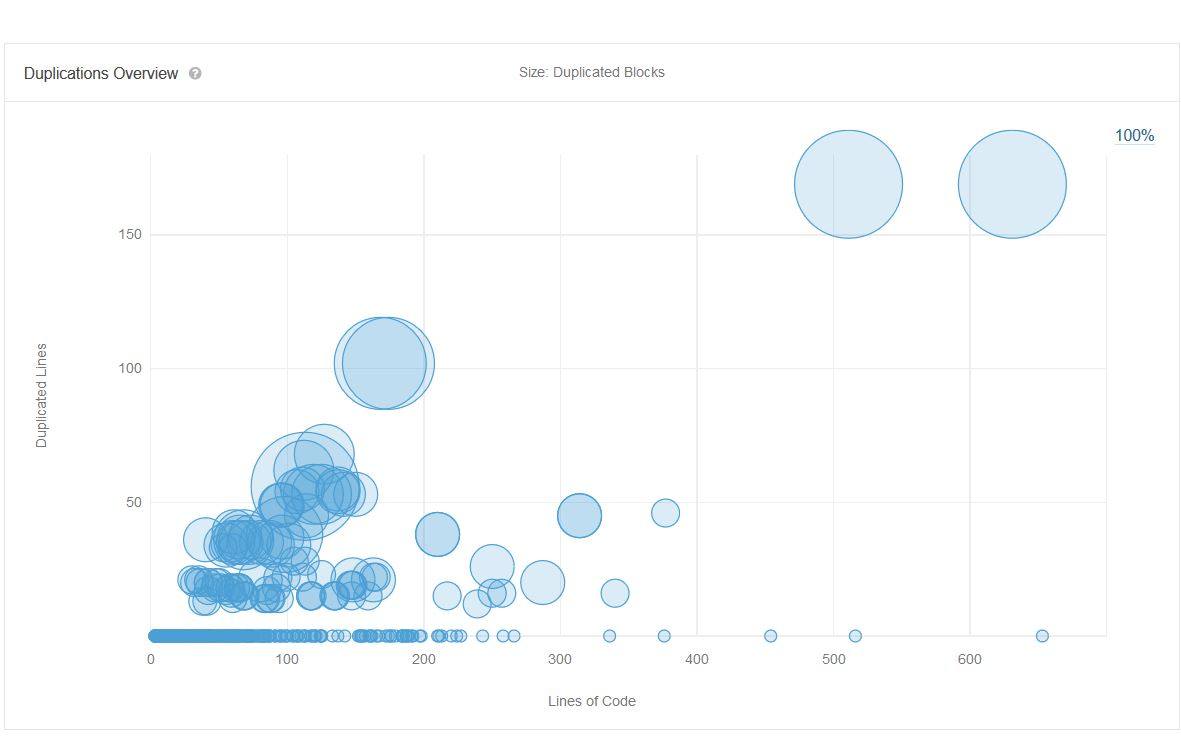
\includegraphics[scale=1]{figures/duplicatedlines.JPG}
                \caption{Overview of the occurences of duplicated lines\\
                        Vertical: the number of duplicated lines found in a class\\
                        Horizontal: the number of lines of code in a class}
                \label{fig:duplicatelines}
            \end{figure}
            
            From the figure, we find the following: 
            \begin{itemize}
                \item[-] There is a high number of duplicated LOC in two big files. They both have 169 duplicated LOC contained in 6 blocks. Those two classes are: 
                \begin{enumerate}
                    \item \cb{core/config/heuristic/selector/value/ValueSelectorConfig.java}\\
                    In this file, 22.7\% of the lines of code are duplicates. 
                    \item \cb{core/config/heuristic/selector/entity/EntitySelectorConfig.java}\\
                     In this file, 27.3\% of the lines of code are duplicates. 
                \end{enumerate}
                \item[-] Two other classes stand out, with 105 duplicate lines contained in 5 blocks. 
                \item[-] There is a big number of files that contain 70 duplicated lines or less, with a few big clusters of files around 38 and 25. 
 
            \end{itemize}
            Code duplication could generally be avoided by either extracting a parent class or by using composition. In some cases this is not possible, but since these two blocks of code are so big, we do believe that something can be done to remove the big number of duplicated lines, as we mentioned before. \\
            However, the project that we chose has a rather low number of duplicated lines, given its size and the complexity.
         
        \subsubsection{Code Smells}
            By definition, code smells are characteristics of the code that could possibly indicate a deeper problem. Sometimes, the smells can be rather superficial and only surface issues, such as a variable not following the given naming convention. But other times, code smells can also indicate deeper issues, such as classes that are overly complex or are badly designed. As such, finding these code smells, analysing them and trying to solve them is a good way to ensure that the code is more maintainable and, by solving them early, we could prevent them from evolving into actual bugs. 
            \\ \\
            According to SonarQube, the project has 3,420 total smells, out of which 2,313 are in the \cb{optaplanner-core} package. In total, the accumulated debt of the project is 96 days (meaning that it would take one developer 96 days to fix all of the code smells). However, the debt ratio is very low - only 1.5\%, and because of this, the rating of the project with regards to Maintainability is A. An overview of the distribution of the code smells in the \cb{core} package's three main folders can be seen in Figure \ref{fig:numberofcodesmells}.
            \begin{figure}[H]
                \centering
                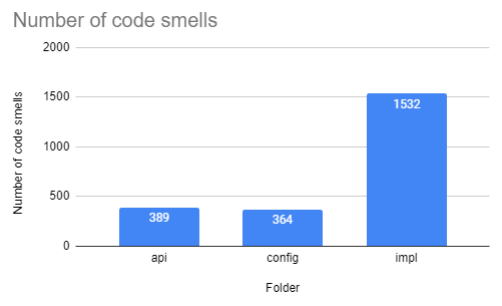
\includegraphics{figures/step4/step4.2/numberofcodesmells.PNG}
                \caption{Distribution of code smells in the \cb{core} package}
                \label{fig:numberofcodesmells}
            \end{figure}
            We expected that, in the \cb{core} package, the \cb{impl} folder should have the most code smells, due to the nature of the code inside this folder, as well as the complexity which we have discussed previously. And indeed, the folder has 1532 code smells, three times as much as each of the other two folders. 
            An overview of the distribution of code smells inside the \cb{core.impl} folder can be seen in Figure \ref{fig:codesmellimpl}.
            \begin{figure}[H]
                \centering
                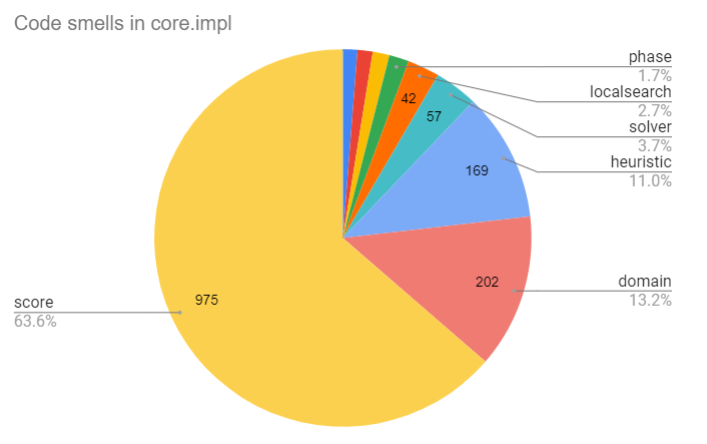
\includegraphics[scale=0.8]{figures/step4/codesmellsimpl.PNG}
                \caption{Caption}
                \label{fig:codesmellimpl}
            \end{figure}
            When analysing the code smells and further investigating what they are and where they occur, we have found the following: 
            \begin{itemize}
                \item The first smell that we have come across was the fact that a generic variable contained an unexpected character. When looking through the project, we observed that the developers hold a certain convention when typing generics, namely using the character \cb{$\_$} at the end of a variable, like so: \cb{variable$\_$}. This has been picked up by SonarQube as a code smell, and it is quite present everywhere in the project where generics are declared or used. Figure \ref{fig:smell4} gives an example of such an occurrence: 
                \begin{figure}[H]
                    \centering
                    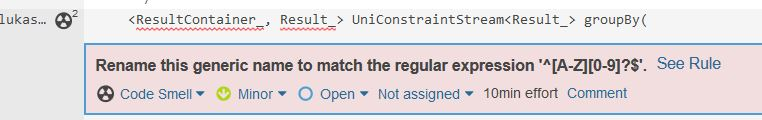
\includegraphics{steps/smell4.JPG}
                    \caption{Variable name containing unexpected character}
                    \label{fig:smell4}
                \end{figure}
                This naming convention can be used to easily distinguish generics from normal variables. After analysing the project we have come to the conclusion that the code relies heavily on generics, and as such, there was a need to distinguish them and to make them stand out more. We believe that this was the main reason behind this unusual naming convention.
                
                \item The file with the most code smells is 
                \cb{core/config/score/director/ScoreDirectorFactoryConfig.java}, which has 86 code smells. Out of those, there are a few \texttt{TODO} comments which are also picked up as smells, or another smell which found that a generic name contains some unusual characters. However, about 80 of the code smells in this class have to do with the fact that deprecated code is being used, and not correctly annotated. \\
                This problem occurs very often when software evolves quickly and different components evolve faster than others; the code tends to change very quickly, and those changes are difficult to track everywhere in the code. As such, some variables or blocks of code become deprecated, not longer needed or used but still present because they were not updated at the right time. 
                \item \textit{Deprecated code should be removed} and \textit{Deprecated elements should have both the annotation and the Javadoc tag} are possibly the most encountered code smells. An example of such a smell occurring can be seen in Figure \ref{smell3}
                \begin{figure}[H]
                    \centering
                    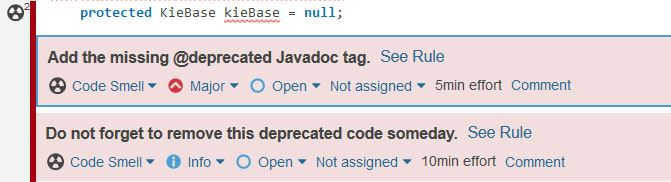
\includegraphics[scale=1.35]{figures/codesmell3.JPG}
                    \caption{Code smell: deprecated variables}
                    \label{fig:smell3}
                \end{figure}
                
                \item The file with the second most code smells is 
                \cb{core/config/localsearch/decider/acceptor/AcceptorConfig.java}. As with the previous file, most of the smells are related to deprecated values or code still being used. However, this file also has a few other smells, such as a function having too high cognitive load, as can be seen in Figure \ref{fig:smells2}, or removing commented out code, as can be seen in Figure \ref{fig:smells1}
                \begin{figure}[H]
                    \centering
                    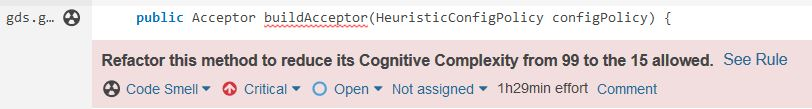
\includegraphics[scale=1.4]{figures/smell2.JPG}
                    \caption{Code smells: Function with a high cognitive load}
                    \label{fig:smells2}
                \end{figure}
                \begin{figure}[H]
                    \centering
                    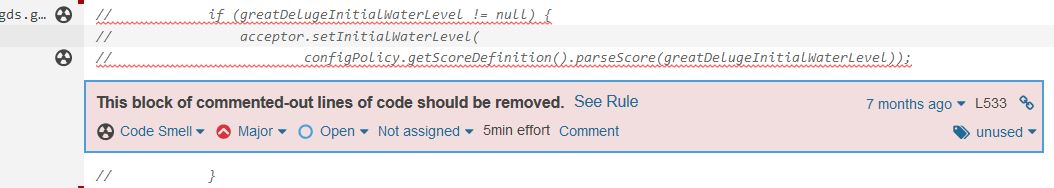
\includegraphics[scale=1.2]{figures/smell1.JPG}
                    \caption{Code smell: Not removing commented out code}
                    \label{fig:smells1}
                \end{figure}
                \item Looking deeper into the code, we have found that there is one folder which has considerably more smells than the rest. There was not one file having the majority of the smells, but they were rather spread out in the files in this particular location: 
                \cb{core/score/stream/drools} had 619 code smells, more than 40\% of the total smells found in the \cb{core} package. Most of the smells found in this location are the same as the ones detected in the previously mentioned files. However, we encountered a different smell here, namely: \textit{Functional Interfaces should be as specialised as possible}. The occurrence can be seen in Figure \ref{fig:smell5}. It is marked as minor, and it would need very little effort to solve, by simply using a specialsed interface instead of a general one.
                \begin{figure}[H]
                    \centering
                    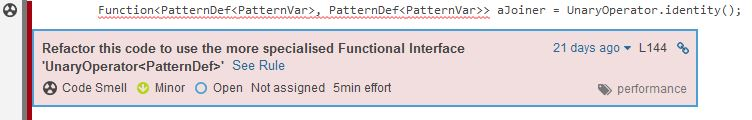
\includegraphics[scale=1.5]{figures/smell5.JPG}
                    \caption{Code smell: Not using specialised interfaces}
                    \label{fig:smell5}
                \end{figure}
            \end{itemize}
            
        \subsubsection{Bugs}
            Despite the high number of code smells in the codebase, we have found that there are very few bugs for a project of this size. In total, the project only has 46 bugs.
            \begin{enumerate}
                \item \textbf{Critical bugs}\\
                In the whole project there was only one critical bug - a division by 0 which was not entirely checked. The tool was very good in capturing this bug. The piece of code responsible can be seen in Figure \ref{fig:criticalbug}. The estimated time required to solve this bug is approximately 5 minutes - so the developers should have this as a very high priority on the TODO list.
                \begin{figure}[H]
                    \centering
                    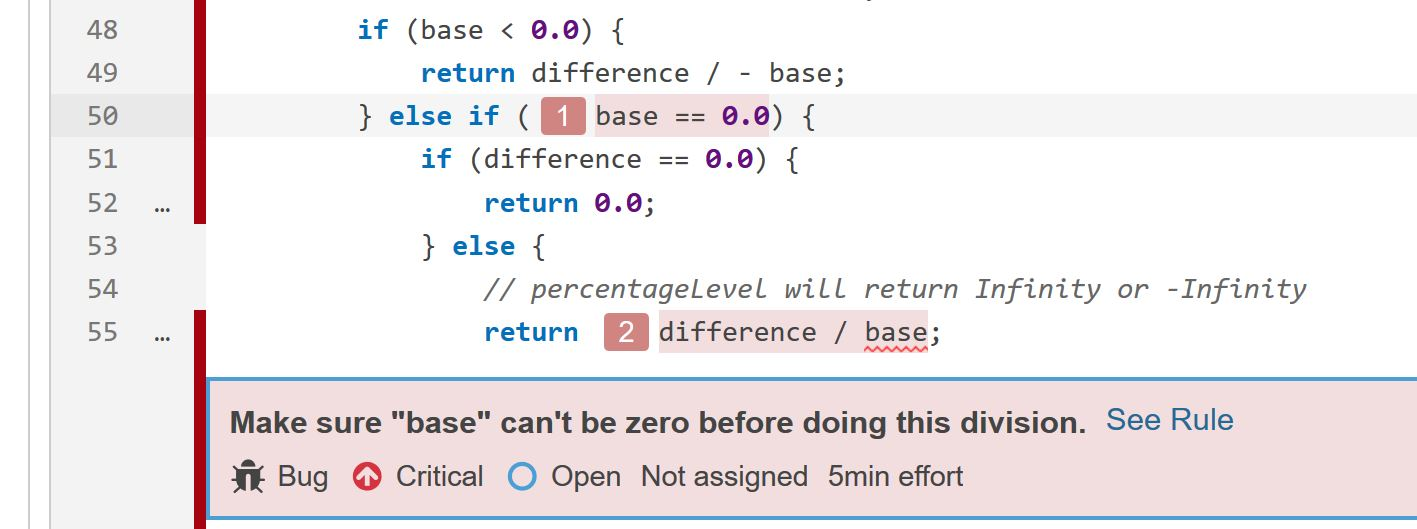
\includegraphics[scale=0.8]{figures/criticalbug.JPG}
                    \caption{The only critical bug found in the whole project.}
                    \label{fig:criticalbug}
                \end{figure}
                
                \item \textbf{Major bugs}\\
                In total, there were 13 major bugs in the project. Six of them can be found in the class: \cb{core/api/score/stream/Joiners.java}, and they are all concerned with the same bug: the developers gave a method a reserved name without mentioning if it is an override - and this can cause unexpected behavior. An example of such an occurrence can be seen in Figure \ref{fig:majorbug}. The rest of the major bugs were of similar nature.
                \begin{figure}[H]
                    \centering
                    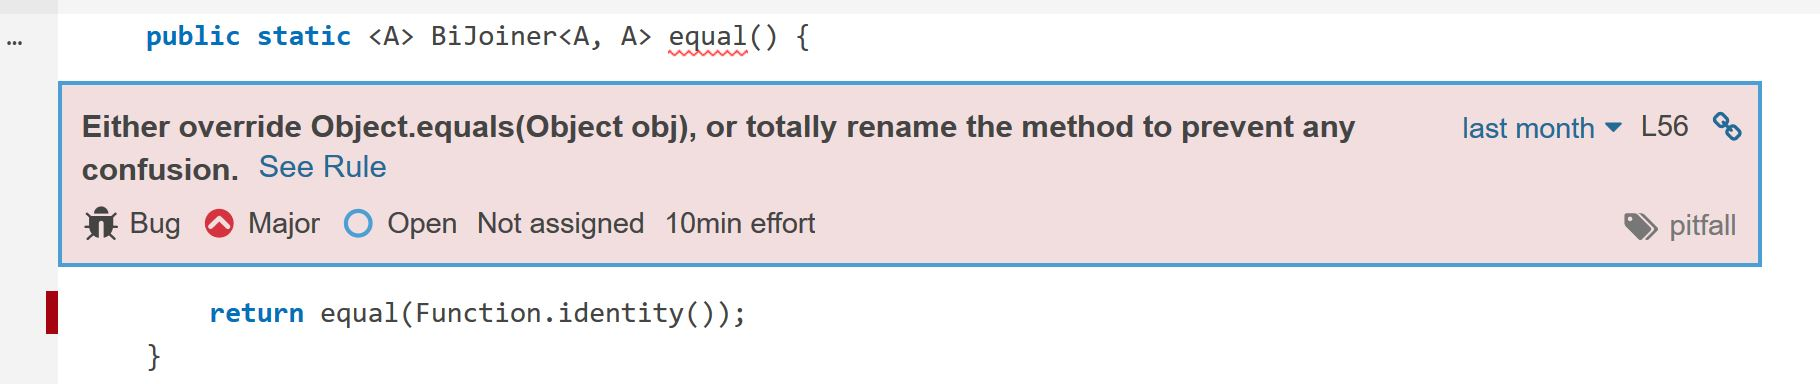
\includegraphics[scale=0.8]{figures/majorbug.JPG}
                    \caption{An example of a major bug}
                    \label{fig:majorbug}
                \end{figure}
                
                \item \textbf{Minor bugs}\\
                The project had a total of 32 minor bugs. The class with the most bugs had 6, and they were all concerned with the missing typecasting of variables when performing arithmetical operations. Two such examples can be seen in Figure \ref{fig:minorbugs}.
                \begin{figure}[H]
                    \centering
                    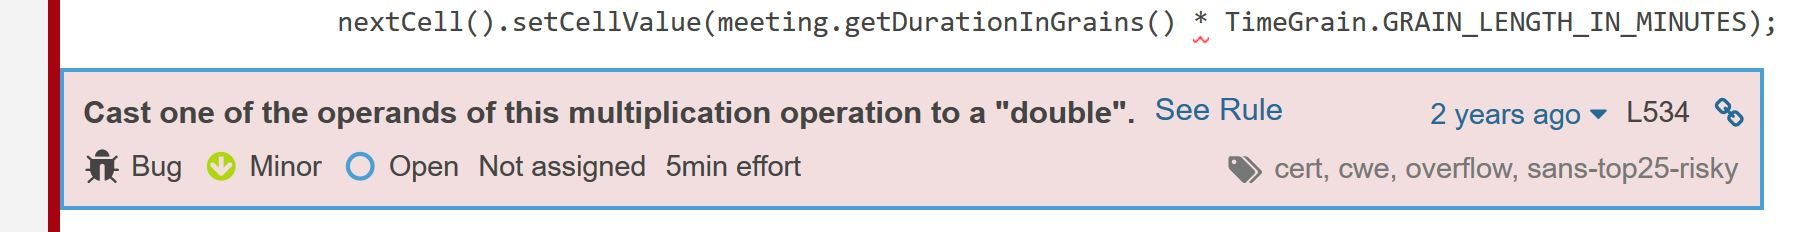
\includegraphics[scale=0.8]{figures/minorbug.JPG}
                    \caption{Example of a minor bug}
                    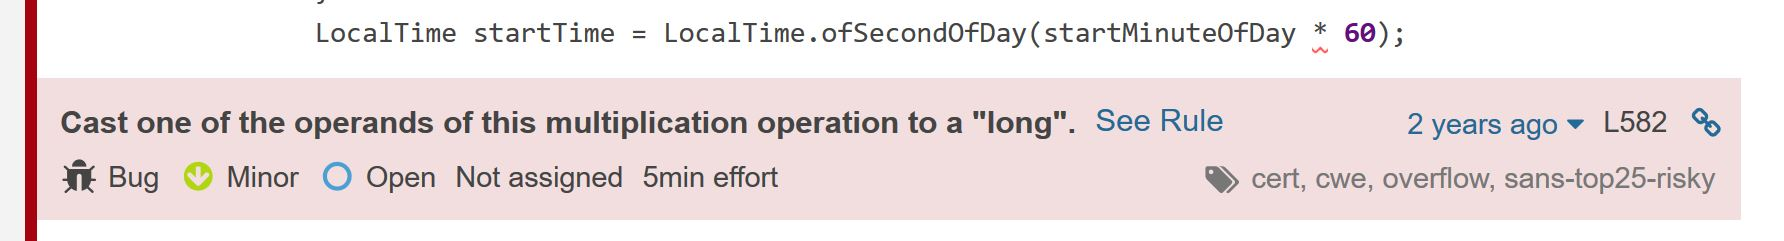
\includegraphics[scale=0.8]{figures/minorbug2.JPG}
                    \caption{Examples of minor bug}
                    \label{fig:minorbugs}
                \end{figure}
            \end{enumerate}
            
            As mentioned before, we believe that the severity of these bugs together with the relatively low number indicate a very good code quality and that the developers should strive to continuously maintain the project in order to adhere to the same high standards.
        
        \subsubsection{Coverage}
            According to the tool, our analysed software has 0\% coverage, meaning that there are no unit tests whatsoever and that none of the classes/modules/methods are tested. Investigating why this could happen, we have come up with the following possible reasons:
            \begin{enumerate}
                \item The tool is looking for line-coverage, meaning that, for every line of code, it is searching for a test method that will cover it. Our software does not have this kind of testing, but only functional tests which handle the behaviour of an entire module. \\
                For example, the test class \texttt{SimpleScoreVerifier.java} tests whether the score of a solution has the expected weight after being computed. \\
                The fact that our software only has some partial functional testing, it could be that the tool did not pick them up when analysing the coverage.
                \item The test classes are placed in a different package called \texttt{optaplanner-test}, separately from the \texttt{core} package which contains the implementation. As such, it could be that SonarQube did not pick up the connection between the tests and the code. The documentation did not have any other useful information about this, so we could assume that this could have been a reason why the coverage was 0, since usually the tests should be placed in the same package as the code.
            \end{enumerate}
            